%%%%%%%%%%%%%%%%%%%%%%%%%%%%%%%%%%%%%%%%%
% Arsclassica Article
% LaTeX Template
% Version 1.1 (1/8/17)
%
% This template has been downloaded from:
% http://www.LaTeXTemplates.com
%
% Original author:
% Lorenzo Pantieri (http://www.lorenzopantieri.net) with extensive modifications by:
% Vel (vel@latextemplates.com)
%
% License:
% CC BY-NC-SA 3.0 (http://creativecommons.org/licenses/by-nc-sa/3.0/)
%
%%%%%%%%%%%%%%%%%%%%%%%%%%%%%%%%%%%%%%%%%

%----------------------------------------------------------------------------------------
%	PACKAGES AND OTHER DOCUMENT CONFIGURATIONS
%----------------------------------------------------------------------------------------

\documentclass[
10pt, % Main document font size
a4paper, % Paper type, use 'letterpaper' for US Letter paper
oneside, % One page layout (no page indentation)
%twoside, % Two page layout (page indentation for binding and different headers)
headinclude,footinclude, % Extra spacing for the header and footer
BCOR5mm, % Binding correction
]{scrartcl}

%%%%%%%%%%%%%%%%%%%%%%%%%%%%%%%%%%%%%%%%%
% Arsclassica Article
% Structure Specification File
%
% This file has been downloaded from:
% http://www.LaTeXTemplates.com
%
% Original author:
% Lorenzo Pantieri (http://www.lorenzopantieri.net) with extensive modifications by:
% Vel (vel@latextemplates.com)
%
% License:
% CC BY-NC-SA 3.0 (http://creativecommons.org/licenses/by-nc-sa/3.0/)
%
%%%%%%%%%%%%%%%%%%%%%%%%%%%%%%%%%%%%%%%%%

%----------------------------------------------------------------------------------------
%	REQUIRED PACKAGES
%----------------------------------------------------------------------------------------

\usepackage[
nochapters, % Turn off chapters since this is an article        
beramono, % Use the Bera Mono font for monospaced text (\texttt)
eulermath,% Use the Euler font for mathematics
pdfspacing, % Makes use of pdftex’ letter spacing capabilities via the microtype package
dottedtoc % Dotted lines leading to the page numbers in the table of contents
]{classicthesis} % The layout is based on the Classic Thesis style

\usepackage{arsclassica} % Modifies the Classic Thesis package

\usepackage[T1]{fontenc} % Use 8-bit encoding that has 256 glyphs

\usepackage[utf8]{inputenc} % Required for including letters with accents

\usepackage{graphicx} % Required for including images
\graphicspath{{Figures/}} % Set the default folder for images

\usepackage{enumitem} % Required for manipulating the whitespace between and within lists

\usepackage{lipsum} % Used for inserting dummy 'Lorem ipsum' text into the template

\usepackage{subfig} % Required for creating figures with multiple parts (subfigures)

\usepackage{amsmath,amssymb,amsthm} % For including math equations, theorems, symbols, etc

\usepackage{varioref} % More descriptive referencing

%----------------------------------------------------------------------------------------
%	THEOREM STYLES
%---------------------------------------------------------------------------------------

\theoremstyle{definition} % Define theorem styles here based on the definition style (used for definitions and examples)
\newtheorem{definition}{Definition}

\theoremstyle{plain} % Define theorem styles here based on the plain style (used for theorems, lemmas, propositions)
\newtheorem{theorem}{Theorem}

\theoremstyle{remark} % Define theorem styles here based on the remark style (used for remarks and notes)

%----------------------------------------------------------------------------------------
%	HYPERLINKS
%---------------------------------------------------------------------------------------

\hypersetup{
%draft, % Uncomment to remove all links (useful for printing in black and white)
colorlinks=true, breaklinks=true, bookmarks=true,bookmarksnumbered,
urlcolor=webbrown, linkcolor=RoyalBlue, citecolor=webgreen, % Link colors
pdftitle={}, % PDF title
pdfauthor={\textcopyright}, % PDF Author
pdfsubject={}, % PDF Subject
pdfkeywords={}, % PDF Keywords
pdfcreator={pdfLaTeX}, % PDF Creator
pdfproducer={LaTeX with hyperref and ClassicThesis} % PDF producer
}
 % Include the structure.tex file which specified the document structure and layout

\usepackage{tikz}
\usepackage{tikzscale}
\usepackage{pgfplots}
\usepackage{xcolor}
\usepackage{graphicx}
\usepackage{amsmath}
\usetikzlibrary{snakes,arrows,shapes}
\usetikzlibrary{arrows.meta}
\DeclareMathOperator*{\argmax}{arg\,max}
\DeclareMathOperator*{\argmin}{arg\,min}

%----------------------------------------------------------------------------------------
%	TITLE AND AUTHOR(S)
%----------------------------------------------------------------------------------------

\title{\normalfont\spacedallcaps{Oral Presentation Summary}} % The article title

\subtitle{In requirement for PhD program} % Uncomment to display a subtitle

\author{\spacedlowsmallcaps{Mark Burgess}} % The article author(s) - author affiliations need to be specified in the AUTHOR AFFILIATIONS block

%\date{} % An optional date to appear under the author(s)

%----------------------------------------------------------------------------------------

\begin{document}

%----------------------------------------------------------------------------------------
%	HEADERS
%----------------------------------------------------------------------------------------

\renewcommand{\sectionmark}[1]{\markright{\spacedlowsmallcaps{#1}}} % The header for all pages (oneside) or for even pages (twoside)
%\renewcommand{\subsectionmark}[1]{\markright{\thesubsection~#1}} % Uncomment when using the twoside option - this modifies the header on odd pages
\lehead{\mbox{\llap{\small\thepage\kern1em\color{halfgray} \vline}\color{halfgray}\hspace{0.5em}\rightmark\hfil}} % The header style

\pagestyle{scrheadings} % Enable the headers specified in this block

%----------------------------------------------------------------------------------------
%	TABLE OF CONTENTS & LISTS OF FIGURES AND TABLES
%----------------------------------------------------------------------------------------

\maketitle % Print the title/author/date block

\setcounter{tocdepth}{2} % Set the depth of the table of contents to show sections and subsections only

\tableofcontents % Print the table of contents

%\listoffigures % Print the list of figures

%\listoftables % Print the list of tables


%----------------------------------------------------------------------------------------
%	AUTHOR AFFILIATIONS
%----------------------------------------------------------------------------------------

\let\thefootnote\relax\footnotetext{\textit{Australian National University, College of Engineering and Computer Science (mark.burgess@anu.edu.au)}}

%----------------------------------------------------------------------------------------

%\newpage % Start the article content on the second page, remove this if you have a longer abstract that goes onto the second page

%----------------------------------------------------------------------------------------
%	INTRODUCTION
%----------------------------------------------------------------------------------------

\section{Introduction}

The Australian electricity system is currently being subjective to technological change, particularly the replacement of fossil fuel generators by solar and renewable energy sources, and the intermittancy of renewable generation technology is driving the need for investigation and implementation of energy storage technologies.
Particularly there is much investigation into the potential of renewable energy resources on distribution networks - or Distributed Energy Resources (DERs) - as a solution of future energy grids.
However there currently does not exist any agreed apon market structure for the participation of DERs in future electricity grids.

The investigation of possible market structures ultimately reduces to a fundamental question "How should electrical energy be traded?", which is identified as having a moral character.
The question of how resources such as money and electricity \textit{should} be distributed between parties is investigated in a branch of philosophy called \textit{Distributive Justice}.
Distributive Justice analyses this question in terms of vague moral elements such as various notions of \textit{Equality}, \textit{Efficiency}, \textit{Deservedness}, \textit{Proportionality}, etc.
But unfortunately most of these vague moral elements conflict amongst themself and do not nessisarily lead to definitive and defined solutions.

Alternatively there exist a range of defined solutions that exist in disparate fields that do can directly give tangible answers to the question of how electrical and monetary resources should be allocated. Particularly:
\begin{enumerate}[noitemsep]
\item From the field of micro-economics comes the description of normative trading established by \textit{Marginalist} principles, particularly the mechanism of 'Locational Marginal Pricing' (LMP)
\item From the field of Mechanism Design comes the description of idealised incentive compatable allocation embodied in the Vickrey Clark Groves (VCG) mechanism.
\item From the field of cooperative Game Theory comes the description of axiomatic allocation in proportion to marginal contribution between possible coalitions, particularly the Shapley Value (SV)
\item From the field of Game Theory comes the description of idealised negotion between small numbers of parties in respect with potential threats they can leverage against each other, particularly Nash Bargaining.
\end{enumerate}

Our development extends the small-numbers limitation in Nash bargaining (point 4) to embody arbitrary numbers of players allocating according to strength of possible coalitions and mirroring SV axioms (point 3).
We then develop this new solution called the \textit{Generalised Neyman \& Kohlberg Value} (or GNK value) and approximate it using sampling theory in the context of larger electricity networks and compare it against the solutions given by LMP and VCG in the same context (points 1\&2).

The results are discussed and compared against these two other solutions, particulary in respect that they satisfy or fail-to satisfy broader moral notions in Distributive Justice.

\subsection{Structure}
The summary is composed of the following sections:

\begin{itemize}[noitemsep]
\item	in Section \ref{}, is discussed the moral nature and intractability of the problem of electricity allocation.
\item	in Section \ref{}, we briefly qualitively overview the alternative solutions of LMP, and VCG and SV, and Nash bargaining
\item	in Section \ref{}, is introduced our GNK value, and its approximation and computation for larger electricity networks.
\item	in Section \ref{}, we discuss and morally compare the results of the methods.
\end{itemize}


\section{Existing Solution Space}

There exist a range of relevent existing solutions which are able to allocate resources in a general context in the presence of monetary transactions.
Particularly these consider a possible span of outcomes usually in terms of utility, and an allocation in this context allocates an outcome and gives a transfer of utility (ie. money) between the participants.
These notable mechnaisms include:

\paragraph{The VCG mechanism}
The VCG mechanism is an allocation process where each player is payed utility equal to the impact that their presence has upon others (ie. their externality) in the decision process which selects an outcome that maximises the sum of utility. let us explain:

The VCG process is a bidding process of $n$ agents over set of outcomes $X$ where every agent $i$ has a valuation (or utility) $v_i$,
($ v_i~:~X\rightarrow \mathbb{R}_{\ge 0} $)\\
The process asks every agent for their valuations and instigates the outcome that maximises the sum of the reported valuations:
$ x^* = \argmax_{x\in X}\sum_{i=1}^{n}v_i(x) $\\
This outcome is implemented and the bidding process pays each agent $i$ the utility value $d_i$ (which may be positive or negative):
\begin{equation}\label{eq:VCG_payment_rule} d_i(v)=\sum_{j\ne i}v_j(x^*) - \max_{x'\in X}\sum_{j\ne i}v_j(x') \end{equation}
And this value $d_i$ is the value that the player's presence adds to the utility of others minus the sum of the other player's utility which would have been obtained in the player's absence - ie. the player's externality.


The most notable property is that the VCG mechanism is to be \textit{truthful} or \textit{incentive compatible}, in that no single player can possibly gain by misreporting their valuations in the event that the utility of the agents is \textit{quasilinear}.\cite{roberts1979characterization, Lavi2008} 
ie. if each player's utility $u_i$ has form:
$ u_i = d_i(v)+v_i $

VCG is also \textit{individual rationality}, in that no agent (assuming quasilinear utility) will ever be left with a net negative utility.
However, one primary drawback of this mechanism is that it is not \textit{budget balanced}, in that it is possible for the amount of utility that is transferred between the players might not sum to zero.


\paragraph{The Shapley Value}

The \textit{Shapley value} is a well known solution concept in cooperative game theory, which allocates to each individual player the average marginal contribution they would add under uncertainty of the presence of other players.

The basic elements of a classic cooperative game are that there is a set of players$N=\{1,2,\dots n\}$ and a function $v: S\subseteq N \rightarrow \mathbb{R}$ with $v(\emptyset)=0$ called the \textit{characteristic function}.
The characteristic function identifies in some sense the `worth' or `value' of any group of players (a `coalition'), and one aim of cooperative game theory is to develop solution concepts which split the wealth achieved if everybody cooperated (that is $v(N)$) between all the players.

Particularly, for any coalition $S$ which does not include a player $i$, then player $i$'s marginal contribution is $v(S\cup\{i\}) - v(S)$. If we average such contributions for coalitions of size $k$:
\begin{equation}\label{eq:shapley_value2}
\hat{v}_{i,k} = \frac{1}{\binom{n-1}{k}}\sum_{S\subseteq N\setminus \{ i\} , |S|=k} %\frac{(n-|S|-1)!\,|S|!}{(n-1)!}
(v(S\cup\{i\})-v(S))
\end{equation}
Then we have the average marginal contribution of player $i$ to coalitions of size $k$, and if we average this over coalitions of different size, we get the Shapley value:
\begin{equation}\label{shap2} \varphi_i(\langle N,v\rangle) = \frac{1}{n}\sum_{k=0}^{n-1}\hat{v}_{i,k} \end{equation}

The shapley value satisfies a range different sets of attractive axioms, such as:
\begin{itemize}
\item	\textbf{Efficiency}: That the total dividend is broken up, $\sum_i\varphi(\langle N,v\rangle)_i = v(N)$
\item	\textbf{Symmetry}: If two players $i$ and $j$ are substitutes and contribute the same to all coalitions, such that if $v(S\cup i)=v(S\cup j)~~\forall S\subseteq N\setminus\{i,j\}$, then $\varphi(\langle N,v\rangle)_i = \varphi(\langle N,v\rangle)_j$
\item	\textbf{Dummy Player}: A player $i$ is a dummy player if the amount that $i$ contributes to any coalition is the amount that $i$ is able to achieve alone (i.e.\ $v(S\cup \{i\})-v(S)=v(\{i\})~~\forall S\subseteq N\setminus\{i\}$) then $\varphi(\langle N,v\rangle)_i=v(\{i\})$
\item	\textbf{Additivity}: That for any two games, the imputation for the two together is the sum of the imputations in each, for any $v_1$ and $v_2$, $\varphi(\langle N,v_1+v_2\rangle)=\varphi(\langle N,v_1 \rangle) + \varphi(\langle N,v_2\rangle)$
\end{itemize}

\paragraph{Locational Marginal Pricing}

Locational Marginal Pricing approach extends from microeconomic theory and thought.
Particularly the utilitarian perspective sought to explain market dynamics in terms of people's efforts to maximise their own utility (or more practically, profit), and in this context stable (and hence normal) market prices were associated with the equilibrium of those efforts.
And this perspective yielded a link between market dynamics with the concept of the margin - or `marginalism'.
Ultimately marginalism was adopted mainstream in the so-called 'marginal revolution', which has been identified (such as by \cite{marginalism1}) as defining the beginning of neoclassical economics.

The marginalist revolution saw that economic prices were not just equal to the summation of normal production costs (ultimately depending on the value of labor), but instead depended on the cost of production of the most marginal unit produced to meet demand.

The idea of marginalism is best illustrated with a graph that might well appear in economic texts, in Figure \ref{fig_demand_supply} there is an illustration of a hypothetical market for a particular economic good, with many suppliers and many buyers.
In the figure we have the plotted the `Supply curve', identifying how many units of the good could be sustainably supplied to the market if the units sold for a particular price.
And we also have the `Demand curve', identifying how many units of the good would natrually be sold depending on the price which the goods sold at.
In this way, if the market is functioning ideally, then there is only one sensible outcome: that the goods should be sold in the number (and therefore at the price), that is at the intersection of the supply and demand curves - ie. the marginal price point.

One of the most notable features of this neoclassical analysis is that the equilibrium marginal price point also maximises the sum of utility of those that participate in the market.
This can be seen from Figure \ref{fig_demand_supply} where all the buyers who value the goods the most are provided from all the sellers who can supply those goods at lowest cost up until the marginal point where no further trade is viable.

This point of utility maximisation is seen in Neoclassical analysis more generally, where market equilibrium prices (at and/or between markets) occur at the point of the maximisation of the sum of utility. Indeed, the process of mathematically deriving these marginal prices developed into a kind of calculus, where the marginal prices fall out as Lagrange multipliers in the process of maximising the sum of utility - these are Locational Marginal Prices.


\begin{figure}[]{}
    \centering
	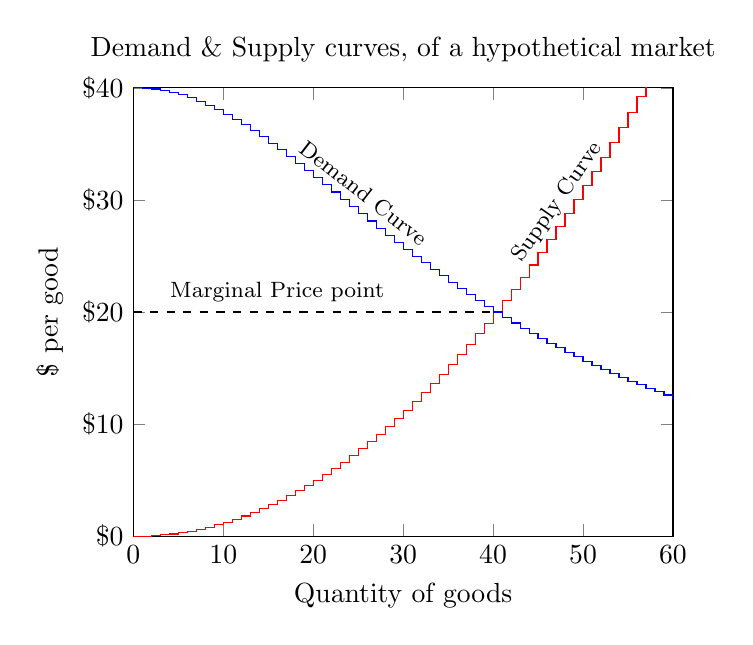
\begin{tikzpicture}
	\begin{axis}[
		title={Demand \& Supply curves, of a hypothetical market},
		xlabel={Quantity of goods},
		ylabel={\$ per good},
		xmin=0, xmax=60,
		ymin=0, ymax=40,
		%xtick={0,0.05,0.1,0.15,0.2,0.25},
		%ytick={30,35,40},
		yticklabel=$\$\pgfmathprintnumber{\tick}$,
		%ymajorgrids=true,
		grid style=dashed,
		xticklabel style={/pgf/number format/fixed},
	]
	\addplot[red] coordinates {
(0,0.0)(1,0.0)(1,0.012500000000000002)(2,0.012500000000000002)(2,0.05000000000000001)(3,0.05000000000000001)(3,0.11249999999999999)(4,0.11249999999999999)(4,0.20000000000000004)(5,0.20000000000000004)(5,0.3125)(6,0.3125)(6,0.44999999999999996)(7,0.44999999999999996)(7,0.6124999999999999)(8,0.6124999999999999)(8,0.8000000000000002)(9,0.8000000000000002)(9,1.0125000000000002)(10,1.0125000000000002)(10,1.25)(11,1.25)(11,1.5125000000000002)(12,1.5125000000000002)(12,1.7999999999999998)(13,1.7999999999999998)(13,2.1125000000000003)(14,2.1125000000000003)(14,2.4499999999999997)(15,2.4499999999999997)(15,2.8125)(16,2.8125)(16,3.2000000000000006)(17,3.2000000000000006)(17,3.6125)(18,3.6125)(18,4.050000000000001)(19,4.050000000000001)(19,4.5125)(20,4.5125)(20,5.0)(21,5.0)(21,5.5125)(22,5.5125)(22,6.050000000000001)(23,6.050000000000001)(23,6.612499999999999)(24,6.612499999999999)(24,7.199999999999999)(25,7.199999999999999)(25,7.8125)(26,7.8125)(26,8.450000000000001)(27,8.450000000000001)(27,9.1125)(28,9.1125)(28,9.799999999999999)(29,9.799999999999999)(29,10.5125)(30,10.5125)(30,11.25)(31,11.25)(31,12.012500000000001)(32,12.012500000000001)(32,12.800000000000002)(33,12.800000000000002)(33,13.612499999999999)(34,13.612499999999999)(34,14.45)(35,14.45)(35,15.3125)(36,15.3125)(36,16.200000000000003)(37,16.200000000000003)(37,17.1125)(38,17.1125)(38,18.05)(39,18.05)(39,19.0125)(40,19.0125)(40,20.0)(41,20.0)(41,21.0125)(42,21.0125)(42,22.05)(43,22.05)(43,23.112499999999997)(44,23.112499999999997)(44,24.200000000000003)(45,24.200000000000003)(45,25.3125)(46,25.3125)(46,26.449999999999996)(47,26.449999999999996)(47,27.612500000000004)(48,27.612500000000004)(48,28.799999999999997)(49,28.799999999999997)(49,30.012500000000006)(50,30.012500000000006)(50,31.25)(51,31.25)(51,32.512499999999996)(52,32.512499999999996)(52,33.800000000000004)(53,33.800000000000004)(53,35.1125)(54,35.1125)(54,36.45)(55,36.45)(55,37.8125)(56,37.8125)(56,39.199999999999996)(57,39.199999999999996)(57,40.612500000000004)(58,40.612500000000004)(58,42.05)(59,42.05)(59,43.5125)(60,43.5125)(60,45.0)(61,45.0)(61,46.51249999999999)(62,46.51249999999999)(62,48.050000000000004)(63,48.050000000000004)(63,49.6125)(64,49.6125)(64,51.20000000000001)(65,51.20000000000001)(65,52.8125)(66,52.8125)(66,54.449999999999996)(67,54.449999999999996)(67,56.1125)(68,56.1125)(68,57.8)(69,57.8)(69,59.51250000000001)(70,59.51250000000001)
		}node[pos=0.6](endofplotsquare){} ;
	\node [above, rotate=55] at (endofplotsquare) {\footnotesize Supply Curve};
	
	\addplot[blue] coordinates {
(0,40.0)(1,40.0)(1,39.97501561524047)(2,39.97501561524047)(2,39.900249376558605)(3,39.900249376558605)(3,39.77625854568055)(4,39.77625854568055)(4,39.603960396039604)(5,39.603960396039604)(5,39.38461538461539)(6,39.38461538461539)(6,39.119804400978)(7,39.119804400978)(7,38.8114008489994)(8,38.8114008489994)(8,38.46153846153846)(9,38.46153846153846)(9,38.0725758477097)(10,38.0725758477097)(10,37.64705882352941)(11,37.64705882352941)(11,37.187681580476465)(12,37.187681580476465)(12,36.69724770642202)(13,36.69724770642202)(13,36.178631995477666)(14,36.178631995477666)(14,35.634743875278396)(15,35.634743875278396)(15,35.06849315068493)(16,35.06849315068493)(16,34.48275862068965)(17,34.48275862068965)(17,33.88035997882477)(18,33.88035997882477)(18,33.26403326403326)(19,33.26403326403326)(19,32.63640999490056)(20,32.63640999490056)(20,32.0)(21,32.0)(21,31.35717785399314)(22,31.35717785399314)(22,30.71017274472169)(23,30.71017274472169)(23,30.061061531235325)(24,30.061061531235325)(24,29.411764705882355)(25,29.411764705882355)(25,28.764044943820224)(26,28.764044943820224)(26,28.1195079086116)(27,28.1195079086116)(27,27.479604980678403)(28,27.479604980678403)(28,26.845637583892618)(29,26.845637583892618)(29,26.218762802130275)(30,26.218762802130275)(30,25.6)(31,25.6)(31,24.990238188207734)(32,24.990238188207734)(32,24.39024390243902)(33,24.39024390243902)(33,23.800669393826702)(34,23.800669393826702)(34,23.222060957910017)(35,23.222060957910017)(35,22.654867256637168)(36,22.654867256637168)(36,22.099447513812155)(37,22.099447513812155)(37,21.55607948804311)(38,21.55607948804311)(38,21.02496714848883)(39,21.02496714848883)(39,20.50624799743672)(40,20.50624799743672)(40,20.0)(41,20.0)(41,19.506248095092957)(42,19.506248095092957)(42,19.024970273483948)(43,19.024970273483948)(43,18.556103218324154)(44,18.556103218324154)(44,18.099547511312217)(45,18.099547511312217)(45,17.655172413793103)(46,17.655172413793103)(46,17.22282023681378)(47,17.22282023681378)(47,16.802310317668677)(48,16.802310317668677)(48,16.39344262295082)(49,16.39344262295082)(49,15.996000999750061)(50,15.996000999750061)(50,15.609756097560975)(51,15.609756097560975)(51,15.234467983813378)(52,15.234467983813378)(52,14.86988847583643)(53,14.86988847583643)(53,14.51576321161261)(54,14.51576321161261)(54,14.171833480956598)(55,14.171833480956598)(55,13.837837837837839)(56,13.837837837837839)(56,13.513513513513514)(57,13.513513513513514)(57,13.198597648999794)(58,13.198597648999794)(58,12.892828364222401)(59,12.892828364222401)(59,12.595945679984254)(60,12.595945679984254)(60,12.307692307692308)(61,12.307692307692308)(61,12.027814320616427)(62,12.027814320616427)(62,11.756061719324025)(63,11.756061719324025)(63,11.49218890285509)(64,11.49218890285509)(64,11.235955056179774)(65,11.235955056179774)(65,10.987124463519313)(66,10.987124463519313)(66,10.745466756212224)(67,10.745466756212224)(67,10.510757102972573)(68,10.510757102972573)(68,10.282776349614396)(69,10.282776349614396)(69,10.06131111460462)(70,10.06131111460462)
		}node[pos=0.35](endofplotsquare){} ;
	\node [above, rotate=-38] at (endofplotsquare) {\footnotesize Demand Curve};


\addplot[dashed] coordinates {
(0,20.0)(40,20.0)
		}node[pos=0.4](endofplotsquare){} ;
	\node [above] at (endofplotsquare) {\footnotesize Marginal Price point};
	\end{axis}
	\end{tikzpicture}
	\vspace{-10pt}
	\caption{The Demand and Supply curves of a hypothetical market.}
	
	\label{fig_demand_supply}
\end{figure}


\paragraph{Bargaining Solution Concepts}

Another class of solutions are the Bargianing solution concepts, notably including the work of John Nash.

Nash bargaining was introduced by John Nash \cite{nash1} as an axiomatic approach to predict the normal result of idealised bargaining over potential outcomes.
It is defined over a set of potential outcomes $F$ % (which might coincide with power-flows and fiscal payments on an electricity network etc.) 
where each of the players $P=\{p_1,p_2,\dots\}$ value the outcomes differently with utilities $u_{p\in P}(f)$ for $f\in F$.
Additionally there is a privileged outcome called the `disagreement' outcome $d$ which represents the event of the negotiation between the players breaking down, and which any player can unilaterally implement.

Nash identified that in this case there is a unique solution satisfying some very intuitive axioms:
\begin{itemize}
\item \textit{Invariant to affine transformations}: that the solution should not change if the utilities of any of the players are scaled (by some positive factor) or offset, ie that they are invariant under the set of affine transformations% that might also represent their relative preferences.
\item \textit{Pareto optimality}: That the solution will not be inferior to any other point in the preferences of all players.
\item \textit{Independence of irrelevant alternatives} (IIA): If any subset of potential outcomes does not feature the solution point or the disagreement point, then it could be removed from consideration without affecting the solution.
\item \textit{Symmetry}: The solution is invariant with regards to the ordering of the players.
\end{itemize}
Nash identified that this solution maximises the product of utilities above the utility of the disagreement point:%\cite{book1}
\begin{equation}\label{nash-product}\text{nash}(F,d) = \argmax_{(f\ge d)\in F}\prod_{p\in P}(u_p(f)-u_p(d))\end{equation}

a singular disagreement outcome may not be very clearly given by the context to begin with.
And so for a Nash bargaining solution concept to be applied, a disagreement outcome must be chosen from the set of possible outcomes, which leads to the question of how this should be done.
In another paper, Nash explicitly addresses the consideration of the agents choosing a disagreement point between themselves in a prior stage in the bargaining process.

Particularly he considers a game specifically between two players, who reach a cooperative outcome in a series of stages of negotiations.
He considers that each of the players has a space of mixed strategies $S_i$ in a normal form game, and for each possible pair of mixed strategies that the players might execute, each receives an immediate payoff $p_1(s_1,s_2)$ and $p_2(s_1,s_2)$ respectively ($s_1\in S_1$, $s_2\in S_2$).
He also considers that there is a set $B$ of possible payoffs for the players if they cooperate, which may be bigger than the set of payoffs in the normal form game.\\
$\text{ie.}\quad \forall s_1\in S_1,s_2\in S_2 \quad (p_1(s_1,s_2), p_2(s_1,s_2)) \in B$

Nash then considers a specific negotiation process:
\begin{enumerate}
\item Each player $i$ chooses a mixed strategy $t_i\in S_i$ that will be used if the two cannot come to an agreement - this is the threat.
\item The players inform each other of their threats.
\item Each player $i$ decides upon a `demand' $d_i$ which is an amount of utility which they will not accept less than, without triggering the chosen threat.
\item If there is a point $(u_1,u_2)$ in B such that $u_1 \ge d_1$, and $u_2 \ge d_2$ (ie. if there is a possible way the demands can be mutually satisifed), then the pay-off to each player $i$ is $d_i$. Otherwise, the pay-off to each player $i$ is given by the result of their threats, $p_i(t_l, t_2)$.
\end{enumerate}

Nash identifies that a natural choice of compatible demands in the second part of the game occurs at the maximising of the Nash product (Equation \ref{nash-product}) above a disagreement point determined by the execution of threat strategies (as elucidated in the previous section \ref{sec:nash_bargaining_exogenous})
Nash then identifies that in light of this result for the second part of the game there exists a unique set of optimal choice of threats $t_i$ for the two players in the first part of the game; which is a Nash equilibrium of them with respect to the subsequent maximisation of the Nash product.


\section{Moral Allocation}

There is a long history of philosophical scepticism about the nature of moral knowledge, and Distributive Justice is not exceptional in this regard.
What is quite evident, is that different people have different incompatable conceptions of how the world should be and that any particular ethical system is likely to be rooted in a specific focus (as encoded by principles, maxims, cultural narrative, language etc) and will yield outcomes that may be disagreeable to some people and agreeable to others.

While we must acknowledge the moral ambiguity inherent in the question of electricity allocation, we contend that this does not mean that any answer is simply as good as any other.
But only that we believe that the suitability of our answer is not something we can totally demonstrate, in principle.
Thus we give a brief overview of some of the elements that feature in people's moral thinking.

\paragraph{Equality}

People tend to believe that they are, should be, or be treated, ‘equal’ in some sense, And this broad conception has changed throughout time and place in history. [Capaldi, 2002]
While the notion that all people `are moral equals' does not nessisarily imply any specifically equal treatment. On a more practical level, the divergences between people's various ideas of equality can be seen as regarding what things should-be equal (when, where and for whom); and also what should be done about inequalities as they may exist.
There are many positions about equality

\paragraph{Formal Equality}

One equality is that people should be subject to systems that treat them in a manner that is impartial. The minimal idea is that an impartial system should not afford arbitrary or unjustified special treatment toward any particular individual/s. Hence that systems should operate by rules which are blind to particular identity and sensitive only to morally relevant characteristics.
And this idea is characteristed by various thought experiments - eg. Rawl’s “Original Position”, Kant’s categorical imperatives, or various positions defined by hypothetical ideal sympathy and/or perfect detachment.

Indeed, by imagination many kinds treatment or processes could be rationalised as being issued by impartial principles which are universally applied. Furthermore, not all kinds of desirable impartiality are mutually compatible, or perfectly achievable in practical settings.
formal equality can be seen as a basic doctrine that ascribes value to the incorporating degrees (and/or kinds) of impartiality into the design of social processes from the outset.

\paragraph{Equality of Social Goods}

Equality can be construed as society wide vague measures such as 'opportunity', 'wealth', 'welfare', 'opportunity for welfare', 'freedom' etc.
but these are to exansive for us to engineer directly against.

\paragraph{Efficiency}

It is occasionally thought that what is morally good for society should have some relationship with what is good for the individuals of society; and there is a question about how to characterise that relationship.
Historically what is morally good for individuals has been associated with such things as happiness \cite{burns2005happiness} or subjective welfare \cite{10.2307/2264894}, access to resources (such as electrical power) \cite{10.2307/2265047}, and/or opportunity for welfare \cite{10.2307/4320203}.
It is useful to illustrate the question by introducing the concept of utility as a quantification of what is good for individuals.

Pareto optimality is one commonly discussed and formalised efficiency condition, and is a property which we satisfy in our subsequent developments.
But there are other measures of efficiency of allocation.

\paragraph{Proportionality by reference point}

examples of proporitionality statements:
\begin{itemize}
\item	punishment proportional to the crime
\item	pay proportional to contribution to the firm
\item	conpensation proportional to damages
\end{itemize}
examples of reference points:
\begin{itemize}
\item	where a business transaction (such as pay for an employee's work) is considered justified if it was attained by a process of truly-free negotiation between the parties, such as to make all parties better off than they would be otherwise.
\item	mill's harm principle
\end{itemize}


\section{The GNK value}


The question then is how to logically and consistently extend Nash's bargaining solution with endogenous disagreement point to an arbitrary number of players.
The fundamental idea behind our approach was first detailed by John Harsanyi in 1963 \cite{values3}.


We begin by considering \cite{KOHLBERG2018139}'s \textit{coalitional game of threats}, 
which is a coalitional game defined by a pair $\langle N,v \rangle$ in which:
\begin{itemize}
\item	$N=\{1,\dots,n\}$ is a finite set of \textit{players} or \textit{agents}, and
\item	$v:2^N\rightarrow \mathbb{R}$ is a \textit{characteristic function} with 
\begin{equation}
v(S)=-v(N\setminus S) \label{myeq2} \quad \forall S\subseteq N.
\end{equation}
\end{itemize}
The intuition for \eqref{myeq2} is that the characteristic function of this game is an measure of the strength of the bargaining position (the `threat' or `advantage') that a coalition, $S$, has over its complement, $N\setminus S$.

It is proven that if $\mathbb{D}$ is the set of all such games, then there exists a unique mapping $\varphi:\mathbb{D}\rightarrow\mathbb{R}^n$ that satisfies the following four axioms:

\begin{itemize}
\item	\textbf{Efficiency}: $\sum_i\varphi(\langle N,v\rangle)_i = v(N)\qquad\qquad\qquad\qquad\qquad\qquad\qquad\qquad\qquad~~\refstepcounter{equation}(\theequation)\label{myeq}$
\item	\textbf{Symmetry}: If two players $i$ and $j$ are substitutes, such that if $v(S\cup i)=v(S\cup j)~~\forall S\subseteq N\setminus\{i,j\}$, then $\varphi(\langle N,v\rangle)_i = \varphi(\langle N,v\rangle)_j$
\item	\textbf{Null Player}: If a player $i$ is a null player (i.e.\ $v(S\cup i)=v(S)~~\forall S\subseteq N$) then $\varphi(\langle N,v\rangle)_i=0$
\item	\textbf{Additivity}: for any $v_1$ and $v_2$, $\varphi(\langle N,v_1+v_2\rangle)=\varphi(\langle N,v_1 \rangle) + \varphi(\langle N,v_2\rangle)$
\end{itemize}

Letting agent $i$'s element of $\varphi$ be denoted by $\varphi_i$, this mapping is:
\begin{equation}\label{da_value_eq} 
\varphi_i(\langle N,v\rangle)
= \frac{1}{n}\sum_{k=1}^n v_{i,k} 
= \frac{1}{n}\sum_{k=1}^n \frac{1}{\binom{n-1}{k-1}} \sum_{\substack{S:i\in S \\ |S|=k}}v(S) 
\end{equation}
Where $v_{i,k}$ is the average value of $v(S)$ for all coalitions of size $k$ that include $i$.
This mapping gives a distribution of the total surplus $v(N)$ among the players, and \cite{KOHLBERG2018139} appropriately call this unique mapping the `Shapley Value' of the game of threats as it mirrors the classic \textit{Shapley Value} of cooperative game theory \cite{Shapley1953a}.

Indeed \cite{KOHLBERG2018139} have shown that for any game of threats $\langle N,v\rangle$ there is a classic cooperative game $\langle N,v'\rangle$ where the two Shapley values are the same.
It is possible to map a game of threats $v$ to a cooperative game $v'$ via relation:
\begin{equation}\label{convert1}
v'(S)=\frac{1}{2}v(S)+\frac{1}{2}v(N)
\end{equation}


We define the characteristic function $v(S)$, in the context of a \textit{generalized non-cooperative game} which is a game where the strategies available to one player may be restricted by the strategy choice of others.
A generalised non-cooperative game consists of a triplet $G = \langle N,A,u \rangle$ in which:
\begin{itemize}
\item	$N=\{1,\dots,n\}$ is a finite set of players,
\item	$A\subseteq \prod_{i\in N}A^i$ is a set of all possible joint strategies, where $A^i$ denotes the set of strategies available to player $i\in N$, and $A$ is a subset of their product space
\item	$\{u_i(a) : A\rightarrow \mathbb{R}\}_{i\in N}$ is a set of functions of each player's payoff/utility when joint strategy $a\in A$ is executed.
\end{itemize}

In this context, we wish to describe the payoff `threat' or `advantage' $v(S)$ of a coalition $S\subseteq N$ (letting $A^S=\prod_{i\in S}A^i$), taking into account the constraints that apply to the joint action space.
Denoting $(x,y)\in A$ as a partition of a joint action between two coalitions $S$ and $N\setminus S$, 
the characteristic function for the game of threats with generalised action spaces is given by:
\begin{align}
\label{knvalue1}
v(S) = &
\frac{1}{2}\min_{\substack{y\in A^{N\setminus S} \\ \text{s.t.}\exists x,(x,y)\in A}} 
\max_{\substack{x\in A^S \\ \text{s.t.}(x,y)\in A}}
	\left(\sum_{i\in S} u_i(x,y) - \sum_{i\in N\setminus S}u_i(x,y)\right)\nonumber\\
+&
\frac{1}{2}\max_{\substack{x\in A^S \\ \text{s.t.}\exists y,(x,y)\in A}}
\min_{\substack{y\in A^{N\setminus S} \\ \text{s.t.}(x,y)\in A}}
	\left(\sum_{i\in S} u_i(x,y) - \sum_{i\in N\setminus S} u_i(x,y) \right)
\end{align}

The requisite condition $v(S)=-v(N\setminus S)$, as given in~\eqref{myeq2}, is immediately satisfied, and \eqref{knvalue1} is a feasible representation of the competitive advantage (or threat) that a coalition has over its complement in a generalised strategy space.
With the characteristic function \eqref{knvalue1}, the formulation of $\varphi$ (per \eqref{da_value_eq}) defines the GNK value.
This is a novel extension of existing work to the space of generalised games (see Section~\ref{relating_to_the_old}).

\section{Application to Electricity Networks}


We begin by setting out the elements of an electricity network under DC approximation:
\begin{itemize}
    \item A set of buses $B$ with, for all $i\in B$:
    \begin{itemize} 
        \item Power consumption at each bus $p_i$, and 
        \item A bus voltage phase-angle $\theta_i$,
    \end{itemize}
    \item Lines $C\subseteq B\times B$, with, for all $(i,j)\in C$: 
        \begin{itemize} 
        \item Line susceptance $b_{i,j}$, and 
        \item Power flow $p_{i,j}$ (power from bus $i$ to $j$), with $p_{i,j}=-p_{j,i}$. 
    \end{itemize}
\end{itemize}
In this context, the DC approximated powerflow constraints (per \cite{Wang1}) are expressed as follows:
\begin{equation}
\label{dcopf1}
\begin{aligned}
\text{DC-powerflow} \quad& \\
\text{Variables:} \quad&  p_{i\in B},\ \theta_{i\in B},\ p_{(i,j)\in C} \\
\text{constraints:} \quad& p_i^{l}\le p_i \le p_i^{u} \\
&p_{i,j}^l \le p_{i,j} \le p_{i,j}^u \\
&p_j = \sum_{(i,j)\in C}p_{i,j}\\
&p_{i,j} = -b_{i,j}(\theta_i - \theta_j)
\end{aligned}
\end{equation}
where $p_i^{l}$, $p_i^{u}$, $p_{i,j}^l$, $p_{i,j}^u$ are the upper and lower bounds on power consumption/generation and line limits, respectively.


\resizebox*{0.5\columnwidth} {!} {
    \begin {tikzpicture}
		\draw[line width=3pt] (0,0) -- (4,0);
		\draw[line width=3pt] (-2,-3) -- (2,-3);
		\draw[-{Latex[length=5mm, width=4mm]},line width=3pt] (-1,-3) -- (-1,-4);
		\draw[line width=3pt] (1,-4) -- (5,-4);
		\draw[-{Latex[length=5mm, width=4mm]},line width=3pt] (2,-4) -- (2,-5);
		\draw[line width=3pt] (4,-5) -- (8,-5);
		\draw[-{Latex[length=5mm, width=4mm]},line width=3pt] (5,-5) -- (5,-6);
		\draw[line width=3pt] (2,-7) -- (6,-7);
		\draw[-{Latex[length=5mm, width=4mm]},line width=3pt] (3,-7) -- (3,-8);

		\draw[line width=1pt] (1,0) -- (1,-1);
		\draw[line width=1pt] (1,-1) -- (0,-2);
		\draw[line width=1pt] (0,-2) -- (0,-3);

		\draw[line width=1pt] (2,0) -- (2,-1);
		\draw[line width=1pt] (2,-1) -- (3,-2);
		\draw[line width=1pt] (3,-2) -- (3,-4);

		\draw[line width=1pt] (3,0) -- (3,-1);
		\draw[line width=1pt] (3,-1) -- (6,-2);
		\draw[line width=1pt] (6,-2) -- (6,-5);
		
		
		\draw[line width=1pt] (3.5,-4) -- (3.5,-7);

		\draw[line width=1pt] (2.2,0) -- (2.2,1);
		\draw (2.2,1.5) circle (0.5);
		\draw (1.9,1.5) .. controls (1.9+0.2,1.5+0.7) and (2.5-0.2,1.5-0.7) .. (2.5,1.5);

		\node (text) at (4.1,0+0.4) {\scalebox{1.9}{1}};
		\node (text) at (2.1,-3+0.4) {\scalebox{1.9}{2}};
		\node (text) at (5.1,-4+0.4) {\scalebox{1.9}{3}};
		\node (text) at (8.1,-5+0.4) {\scalebox{1.9}{4}};
		\node (text) at (6.1,-7+0.4) {\scalebox{1.9}{5}};
    \end {tikzpicture}
}

%----------------------------------------------------------------------------------------
%	METHODS
%----------------------------------------------------------------------------------------

\section{Methods}

\lipsum[5] % Dummy text

\begin{enumerate}[noitemsep] % [noitemsep] removes whitespace between the items for a compact look
\item First item in a list
\item Second item in a list
\item Third item in a list
\end{enumerate}

%------------------------------------------------

\subsection{Paragraphs}

\lipsum[6] % Dummy text

\paragraph{Paragraph Description} \lipsum[7] % Dummy text

\paragraph{Different Paragraph Description} \lipsum[8] % Dummy text

%------------------------------------------------

\subsection{Math}

\lipsum[4] % Dummy text

\begin{equation}
\cos^3 \theta =\frac{1}{4}\cos\theta+\frac{3}{4}\cos 3\theta
\label{eq:refname2}
\end{equation}

\lipsum[5] % Dummy text

\begin{definition}[Gauss] 
To a mathematician it is obvious that
$\int_{-\infty}^{+\infty}
e^{-x^2}\,dx=\sqrt{\pi}$. 
\end{definition} 

\begin{theorem}[Pythagoras]
The square of the hypotenuse (the side opposite the right angle) is equal to the sum of the squares of the other two sides.
\end{theorem}

\begin{proof} 
We have that $\log(1)^2 = 2\log(1)$.
But we also have that $\log(-1)^2=\log(1)=0$.
Then $2\log(-1)=0$, from which the proof.
\end{proof}

%----------------------------------------------------------------------------------------
%	RESULTS AND DISCUSSION
%----------------------------------------------------------------------------------------

\section{Results and Discussion}

Reference to Figure~\vref{fig:gallery}. % The \vref command specifies the location of the reference

%\begin{figure}[tb]
%\centering 
%\includegraphics[width=0.5\columnwidth]{GalleriaStampe} 
%\caption[An example of a floating figure]{An example of a floating figure (a reproduction from the \emph{Gallery of prints}, M.~Escher,\index{Escher, M.~C.} from \url{http://www.mcescher.com/}).} % The text in the square bracket is the caption for the list of figures while the text in the curly brackets is the figure caption
%\label{fig:gallery} 
%\end{figure}

\lipsum[10] % Dummy text

%------------------------------------------------

\subsection{Subsection}

\lipsum[11] % Dummy text

\subsubsection{Subsubsection}

\lipsum[12] % Dummy text

\begin{description}
\item[Word] Definition
\item[Concept] Explanation
\item[Idea] Text
\end{description}

\lipsum[12] % Dummy text

\begin{itemize}[noitemsep] % [noitemsep] removes whitespace between the items for a compact look
\item First item in a list
\item Second item in a list
\item Third item in a list
\end{itemize}

\subsubsection{Table}

\lipsum[13] % Dummy text

\begin{table}[hbt]
\caption{Table of Grades}
\centering
\begin{tabular}{llr}
\toprule
\multicolumn{2}{c}{Name} \\
\cmidrule(r){1-2}
First name & Last Name & Grade \\
\midrule
John & Doe & $7.5$ \\
Richard & Miles & $2$ \\
\bottomrule
\end{tabular}
\label{tab:label}
\end{table}

Reference to Table~\vref{tab:label}. % The \vref command specifies the location of the reference

%------------------------------------------------

\subsection{Figure Composed of Subfigures}

Reference the figure composed of multiple subfigures as Figure~\vref{fig:esempio}. Reference one of the subfigures as Figure~\vref{fig:ipsum}. % The \vref command specifies the location of the reference

\lipsum[15-18] % Dummy text

%\begin{figure}[tb]
%\centering
%\subfloat[A city market.]{\includegraphics[width=.45\columnwidth]{Lorem}} \quad
%\subfloat[Forest landscape.]{\includegraphics[width=.45\columnwidth]{Ipsum}\label{fig:ipsum}} \\
%\subfloat[Mountain landscape.]{\includegraphics[width=.45\columnwidth]{Dolor}} \quad
%\subfloat[A tile decoration.]{\includegraphics[width=.45\columnwidth]{Sit}}
%\caption[A number of pictures.]{A number of pictures with no common theme.} % The text in the square bracket is the caption for the list of figures while the text in the curly brackets is the figure caption
%\label{fig:esempio}
%\end{figure}

%----------------------------------------------------------------------------------------
%	BIBLIOGRAPHY
%----------------------------------------------------------------------------------------

\renewcommand{\refname}{\spacedlowsmallcaps{References}} % For modifying the bibliography heading

\bibliographystyle{unsrt}

\bibliography{sample.bib} % The file containing the bibliography

%----------------------------------------------------------------------------------------

\end{document}
